\documentclass[a4paper,12pt]{article}
\usepackage{amsmath}
\usepackage{amssymb}
\usepackage{graphicx}
\DeclareMathOperator*{\E}{\mathbb{E}}

\begin{document}

\title{Pricing A Credit Spread}
\author{Zwimangadzo Mudau}
\date{\today}

\maketitle

\tableofcontents

\section{Introduction}
One of the assumptions in pricing financial instruments is that the there is no default by any counterparty in the transaction. The results obtained from this assumption will only work in an unrealistic world where defaults rates are zero. In the real world, default risk plays an important role and must included in any financial instrument pricing. Default in many instruments is reflected as a \textit{spread} added on top of base price. Investors will demand a higher spread for the assumed risk of default inherent in most derivatives contracts. The default risk is a subset of a larger category known as Credit risk. It is investors' challenge to find ways to manage and reduce this inherent Credit risk. Credit derivatives provide a way to manage this risk, and also to assume it. Various credit derivatives exist in practice with applications in different areas of the financial markets. One popular group of such derivatives is the Credit Default Swap on a single name and its extenstion Basket Credit Swap on a collection of names. The project will focus mainly on pricing the spread on the basket instrument with five underlyings. Key parameters play varying roles in obtaining the spread; namely, \(i\) the number of underlyings, \(ii\) the recovery rate, and \(iii\) the default correlation. The default correlation is perhaps the most important of these and the project will spend some time on unpacking its influence on the spread. Also specified on the contract's term sheet is the type of contract, i.e 1st-to-default, 2nd-to-default, etc. These also have a bearing on the behaviour of the spread as other paraments change. All these will be examined in the various subsections of the project. The pricing is to be implemented through a Monte Carlo simulation approach. This approach has its own advantages and disadvantes but it is proven to outperform the other methods in higher dimensions similar to the case of multiple underlyings. 

\section{Theoretical Background}
\subsection{Default Free Bond}
As can be found in numerous publications, the price of a coupon bearing, default free, bond can be written as follows, 

\begin{equation}
V(t, T_n) = \sum_{i = 1}^nZ(t, T_i)C_i + Z(t, T_n)F
\end{equation}

where $C$ is the coupon payment, $Z(t, T_i)$ is the zero coupon discount factor, and $F$ is the face value (this can be set to one with no loss of generality). 

This equation can be flipped around to obtain the zero coupon bond discount factors while given the coupon bonds' pricces. This is the so-called bootstrapping method and was employed in the project to obtain the risk free discount curve. The resulting equation for the zero coupon discount factors is, 

\begin{equation}
Z(t, T_n) = \frac{V(t, T_n) - \sum_{i = 1}^{n - 1}Z(t, T_i)C_i}{C_n + 1}
\end{equation}

There are $n$ unknowns $Z$ for each known bond price $V$. If there are few bonds' prices, interpolation methods can be employed to obtain the other missing prices. The US Treasure Bills give a close approximation to default free coupon bonds, and these were used to obtain the zero-coupon default free discount factors.

\subsection{Defaultable Bond and Extensions to CDS}
The next logical step would be to incorporate default risk in the discussion of bonds, or any contingent claim instrument. This has been done extensively in the literature, and the price of a risky contingent claim promising to pay unit payoff at maturity $T$, is given by,

\begin{equation}
B(t, T) = \E[e^{-\int_t^{T}r(s)ds}\left(\mathsf{1}_{(\tau > T)} + \mathsf{LGD}(\tau)\mathsf{1}_{(\tau < T)}\right)]
\end{equation}

The expectation is taken against the risk-neutral survival probabilities. $\tau$ is the random time where default occurs and $\mathsf{1}_{(\tau < T)}$ is the indicator function of the default event. This equation can be simply put in words as, the price of a defaultable bond is the expecation value of the discounted future expected cash flows. The exponential is the discounting term, the sum in the brackets is the expected payoff at maturity. 
\newline
This can be extended to the caseof a single name CDS contract, with swap premiums paid on dates $T_i$, $0 \leq i \leq n$. Further, if a constant recovery rate is assumed and no correlation between default and interests rates, the protection and premium legs of the CDS can be shown to become, 

\begin{equation}
A_{def, t} = \mathsf{LGD}\int_{T_0}^{T_n}Z(T_0, u)F(du)
\end{equation}

\begin{equation}
A_{prem, t} = \sum_{i = 1}^{n}s\delta_{i}Z(T_0, T_i)S(T_i)
\end{equation}

where $S(t) = 1 - F(t)$ is the survival probability, and $F(t)$ is the default probability. These have been defined rigourously in literature and their relationship to hazard rates. $s$ is the premium spread for the contract paid by the protection buyer at the dates $T_i$ provided default has not occured as shown by the presence of $S(T_i)$ in the premium leg. $F(du)$  signifies the probability of default in the short time interval $du$ and the integral is taken against all possible $du$ in the life of the contract. Further simplifications can be made on the integral to yield a summation and the equation of the spread can be found by requiring the premium and protection legs have a difference of zero at initiation of the CDS. The equation of the spread then becomes, 

\begin{equation}
s_n = \frac{\mathsf{LGD}\sum_{i = 1}^{n}Z(T_0, T_i)[S(T_i) - S(T_{i - 1})]}{\sum_{i = 1}^{n}\delta_{i}Z(T_0, T_i)S(T_i)}
\end{equation}

This is the equation of the CDS spread when given survival probabilities $S(T_i)$, however, this can also be flipped around to obtain the survival probabilities from the quoted spreads in the market in a bootstapping scheme similarly as in the case of bonds. The formula for the survival probabilities can be found through iterative procedures, and one gets the following result

\begin{equation}
S(T_n) = \frac{\sum_{i = 1}^{n - 1}Z(T_0, T_i)[\mathsf{LGD}S(T_{i - 1}) - \left(\mathsf{LGD} + s_n\right)S(T_i)]}{Z(T_0, T_n)\left(\mathsf{LGD} + s_n\right)} + \frac{S(T_{n - 1})\mathsf{LGD}}{\mathsf{LGD} + s_n}
\end{equation}

The system of linear equation consists of $n$ unknowns in $n$ equations and can thus be solved for the unknowns; if there are few spread prices, these can be interpolated using an exponential function for instance.

\subsection{Hazard Rates} 

Survival and default probabilities, $S(T)$ and $F(T)$, have to be modelled properly in order to obtain a consistent theory of credit risk. There have been numerous attempts in this regards; Merton's structural approach comes up more often in the literatures. This involves modeling the counterparty's assets and applying option's theory to derive a method of obtaining the default probabilities. The other approach is to model default as an exogenous process, driven by forces external to the company's business and modeled as a poisson process. This is the approach adopted in this project. 

Let $\tau$ denote the first arrival time, i.e default time, and $T$ the maturity of the CDS contract. The probability that $\tau$ is before $T$ is given by, 

\begin{equation}
F(T) = P[\tau \leq T] = 1 - P[\tau > T] = 1 - S(T)
\end{equation}

$S(T)$ can be shown to originate from the hazard function $h(t)$, which itselt is closely related to the poisson process of default, as follows, 

 \begin{equation}
S(T) = e^{-\int_0^Th(s)ds}
\end{equation}

$\tau$ follows the process with pdf given by 

$$f(t) = \lambda e^{-\lambda t}$$ 

Where $\lambda$ is the intensity of the process. $\lambda$ and the hazard function ($h(t)$) can be shown to be equal under certain conditions. From the spread's quotes, it is possible to determine the implied survival probabilities (risk-neutral probabilities that is) and from these, under certain simplifying assumptions, it is possible to obtain the term structure of hazard rates. The integral equation for hazard rates poses a problem when it comes to calculating the rates; often there has to be made, simplifying assumption to reduce the complexity of the problem. There are several assumptions that can be made as found in the literature, however the assumption made in this project is that the hazard function $h(t)$ is deterministic and piece-wise constant. The text by \cite{credit} gives another assumption that can be made about the structure of the hazard rates and provides an explanation on how to proceed to obtain solutions, however that can be involved, requiring use of numerical solvers tools to obtain the parametrs. The piece-wise constant assumption is simpler to implement as decribed here. 
Suppose the survival probabilities $S(T_n)$ have been computed, then to obtain the first hazard rate, the integral equation simply becomes, 

$$h_1 = -\frac{lnS(T_1)}{\delta t} $$
 
The second hazard rate becomes, 

$$h_2 = \frac{lnS(T_1) - lnS(T_2)}{\delta t} $$

And finally, for any $n$ 

\begin{equation}
h_n = \frac{lnS(T_{n - 1}) - lnS(T_n)}{\delta t}
\end{equation}

This is the equation for piece-wise contant hazard rates when given survival probabilities. The hazard rates are like forward rates; i.e only applying in a forward interval of time as seen today. To validate the results, a simple check is to confirm that the calculated hazard rates return the implied probabilities that were used to obtain them. Below is a graph showing the calculated hazard rates for one of the names in the basket, 

\begin{figure}[h]

\centering
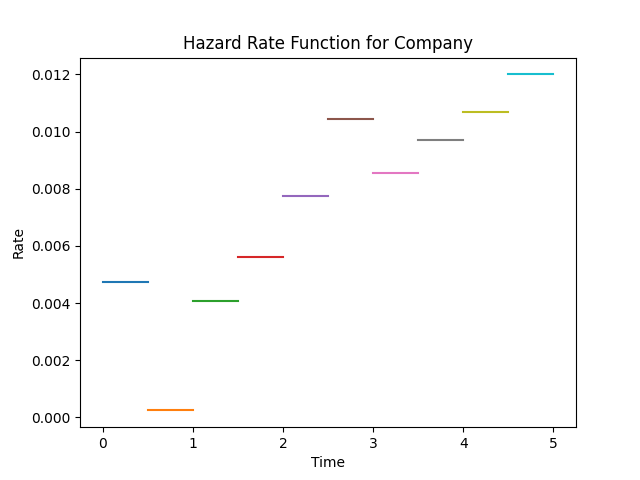
\includegraphics[width=1\textwidth]{hazard_rate_function}
\caption{Piece-Wise Hazard Function}
\label{image-hazard_rate_function}

\end{figure}

\subsubsection{Inverse Cummulative Distributive Function for default time}
Having obtained the hazard rates, it becomes straightforward to get the survival probabilities for any time going into the future. This is obtained through the cdf function for $\tau$, which can be obtained by interpolation techniques on the survival probabilities. However, of rather more important role when it comes to basket cds pricing, is the inverse function of the cdf. There are numerous ways to go about computing inverse cdf for non-normal distributions as mentioned in \cite{peter_jackel}. The approach adopted in this project was to find the collection of hazard rates parameters $h_1, h_2, \dots , h_n$ which give a number close to the given input. Stated more mathematically, suppose $u_i = S(T_i)$ is given, and suppose a constant $\delta t$ where each hazard rate applies, then the goal of the inverse cdf is to find $T_i$ such that 

$$u_i = S(T_i) = e^{-h_1\delta t - h_2 \delta t - \dots - h_n(T_i - t_{n - 1})} $$

The search for $T_i$ is not resource expensive as the functions involved here are the exponential functions only. This at first makes the assumption that $S(T_i)$ is in the range $S(T_1) \leq S(T_i) \leq S(T_n)$, however that can be extended to regions outside this using extrapolation techniques. The procedure above only gives an interval $t_i \leq T_i \leq t_i + \delta t$ where $T_i$ belongs but does not give exact location. To get the exact location, find $T_i$ by gradually incrementing the $t_i$ until the difference , 

$$S(T_i) - e^{-h_1\delta t - h_2 \delta t - \dots - h_{i + 1}(T_i - t_{i})} $$

is close to prescribed accuracy level. 

This gives us the function $S^{-1}(x)$, the inverse cdf for survival, and not $F^{-1}(x)$ the inverse cdf for default. To obtain the latter, the relationship $S(T) = 1 - F(T)$ comes in to lead to the result 

\begin{equation}
F^{-1}(x) = S^{-1}(1 - x)
\end{equation}

\subsection{Basket CDS}
The previous section focused only on single name derivative products. The problem becomes more complex when more than one name are considered. This is coming from the default correlation piece of the puzzle that is introduced when multiple names are involved. Default correlation plays an important role in determining the joint probabilities for default for the basket. In this project the number of underlyings considered was just 5 names, but this can be extended easily to more than that and the problem just takes a while to compute, however the underlying principles are similar. Still adopting notations from the previous sections, one or two more can be added in the case of basket CDS. Let $\tau_i$ denote the default time (random variable) of company $i$ and let $\gamma_n$ denote the default time of the $nth$ name in the basket. $\gamma$ clearly depends on the $\tau_i$'s and the order at which they occur; for a 1st-to-default product, $\gamma_n = min\{\tau_i\}$. The challenge in determining the spread in this case is that the $\tau_i$'s are codependent, meaning that the full joint distribution $P[\tau_1 \leq T, \tau_2 \leq T, \dots, \tau_n \leq T]$ has to be determined. After successful obtaining of the joint cdf the payoff of the basket CDS is then obtained as follows,

\begin{equation}
\E[V_{prem} - V_{pro}] = \int\left(V_{prem} - V_{pro}\right)\psi (\tau_1, \tau_2, \dots, \tau_n)d\tau_1d\tau_2\dots\tau_n
\end{equation}

where $\psi (\tau_1, \tau_2, \dots, \tau_n)$ is the joint default times density, and $V_{prem}$ is given by 

\begin{equation}
V_{prem} = 
\begin{cases} 
\sum\limits_{i = 1}^{j}s\delta t Z(T_i) & \text{if } T_j \leq \gamma_n < T_{j + 1} \leq T \\
\sum\limits_{i = 1}^{m}s\delta t Z(T_i) &  \text{if } \gamma_n > T
\end{cases}
\end{equation}

and $V_{pro}$  is given by, 

\begin{equation}
V_{pro} = \mathsf{LGD}Z(\gamma_n)H(T - \gamma_n)
\end{equation}

where, 

$$ H(T - \gamma_n) = \begin{cases} 1 & \text{if } \gamma_n \leq T \\ 0 & \text{otherwise} \end{cases} $$

Having put the problem in this manner, it immediately becomes clear why Monte Carlo methods are suitable for computation of the spread. This is an expectation problem under multiple factors and this is where Monte Carlo schemes outperform the other numerical techniques. The idea is to simulate $\tau_i$ which follow the distribution (as yet unknown) $\psi(\tau_1, \tau_2, \dots, \tau_n)$ and then take averages of the payoff $V_{prem} - V_{pro}$ at each generated path.
\newline 
The remaining big question is around the functional form of the default density $\psi(\tau_1, \tau_2, \dots, \tau_n)$ and how to obtain it. Luckily, there has been significant development in this area of statistics and with the aid of Sklar's theorem, it is possible to write the cummulative distribution function $\Psi(\tau_1, \tau_2, \dots, \tau_n)$ as a copula on the $\tau_i$'s. Suppose the univariate cdf for each $i$'s name is $F_i(\tau_i)$, then the joint cdf $\Psi(\tau_1, \tau_2, \dots, \tau_n)$ can be written as a copula function of these marginals as follows, 

\begin{equation}
\Psi(\tau_1, \tau_2, \dots, \tau_n) = C(F_1(t), F_2(t), \dots, F_n(t))
\end{equation}

If the $F_i$ are continous and monotonic, then the $F_i^{-1}$ exists, and from known joint distribution (i.e multivariate gaussian or student's t) it is possible to construct copulas as follows, 

\begin{equation}
C(u_1, u_2, \dots, u_n) = F(F_1^{-1}(u_1), F_2^{-1}(u_2), \dots, F_n^{-1}(u_n); \mathbf{\Sigma})
\end{equation}

The project will only look into two copula functions as possible dependent structures for the correlated default times $\tau_i$'s. In both of these the parameter $\mathbf{\Sigma}$ controls the strength of dependence and is calibrated differently for each. 
\newline
Now from the point of view of a protection seller providing protection on a basket of five names, say, the probability of any one of them defaulting is higher than the probability of any two of them defaulting, both events occuring before expiry $T$ and similar default correlation. From this it is not difficult to see why the spread for 1st-to-default basket CDS is higher than that of a 2nd-to-default one. The same argument can be applied to see why the spread for the 2nd-to-default product is greater  than that of the 3rd-to-default, and so on. This will serve as quick check for the Monte Carlo calculations later on.

\section{Numerical Methods}
\subsection{Basic Form Monte Carlo}
The Monte Carlo is itself a numerical method which can include other numerical methods in its process. In this project, these smaller numerical methods came in various forms as outlined in this section. The main skeleton to the Monte Carlo algorithm can be summarized as follows (for the gaussian case, similar algorithm for student's t with just a minute adjustment), as found in the numerous articles referenced here, 

\begin{itemize}
\item Setup a loop $1 \leq j \leq N$
\item Draw $n$ $u_i$ from $U(0, 1)$.
\item Do transformation $z_i = N^{-1}(u_i)$ for all $1 \leq i \leq n$ to obtain $\mathbf{Z}$.
\item With $\mathbf{A}$ $s.t $ $\mathbf{\Sigma} = \mathbf{A}\mathbf{A}^T$, transform $z_i$ to $w_i$ through $\mathbf{W} = \mathbf{A}\mathbf{Z}$.
\item Convert back to $v_i$ through $v_i = N(\mathbf{W_i})$ for each $i$.
\item Obtain simulated $\tau_i$ for each $i$ through $\tau_i = F_i^{-1}(v_i)$. 
\item Calculate $\gamma_n$ depending on type of contract;1st-to-default, 2nd-to-default, etc. and compute the implied $V_{prem}$ and $V_{pro}$ based on $\gamma_n$
\item After all $j$ the spread is $s= \frac{V_{pro}}{V_{prem}}$
\end{itemize}

The first challenge in this algorithm comes when trying to convert the uniform variates $u_i$ into normal variates using $N^{-1}$. When considering lower level programming languages such as C/C++, the task of obtain $N^{-1}$ is not so straightforward. The math library in C++ only includes the error function $erf(x)$, while this is helpful in obtaining the $N(x)$ cummulative normal distribution, it does very little in the case of obtaining the inverse. However, it is possible to obtain approximations to the $erf^{-1}$ using its series approximation formulae.  The link \cite{mimirgames} shows this and some discussions around obtaining the inverse. The equation is, 

\begin{equation}
erf^{-1}(x) = \sum\limits_{k = 0}^{\infty}\frac{c_k}{2k + 1}\left(\frac{\sqrt{\pi}}{2}x \right)^{2k + 1}
\end{equation}

where $c_0 = 1$ and $c_k$ is given by,

$$c_k = \sum\limits_{m = 0}^{k - 1}\frac{c_m c_{k - 1- m}}{(m + 1)(2m + 1)}$$

The approximation is done in practice by choosing where to stop in the summation, as many higher order term are extremely low, and only consume computer memory. The inverse $N^{-1}$ is then obtained from the $erf^{-1}$ using 

$$N^{-1}(x) = \sqrt{2}erf^{-1}(2x - 1)$$

This approach comes with issues when computing the inverse at $x$ close to 1. It is because of this reason that another approach was researched, and one was found in the paper by \cite{sergei}. The nice approximation to the inverse normal $erf^{-1}$ was given as 

\begin{equation}
erf^{-1}(x) = \left[-\frac{2}{\pi a} - \frac{ln(1 - x^2)}{2} + \sqrt{\left(\frac{2}{\pi a} + \frac{ln(1 - x^2)}{2} \right)^2 - \frac{1}{a}}ln(1 - x^2) \right]^{\frac{1}{2}}
\end{equation}

where,

$$a = \frac{8\pi - 24}{12\pi - 3\pi^2}$$

The nice thing about this approximation is its dependence only on the log, root and quadratic functions, all of which are available in the C++ math library. Its error is quite small as compared to the series approximation. Code was written for both functions, but the latter approximation was used going forward. 

The next challenge, minor one, comes in the Cholesky decomposition of the assumed positive definite matrix $\mathbf{\Sigma}$. The method used is a popular one and can be found from various sources, and code was written from scratch, using the formulae,

\begin{equation}
A_{ii} = \sqrt{\Sigma_{ii} - \sum\limits_{k = 1}^{j - 1}A_{ik}^2}
\end{equation}

\begin{equation}
A_{ij} = \frac{1}{A_{jj}}\left( \Sigma_{ij} - \sum\limits_{k = 1}^{j - 1}A_{ik}A_{jk} \right) \text{for } i > j.
\end{equation}

The matrix product $\mathbf{W} = \mathbf{A}\mathbf{Z}$ can be done either from first principles or using libraries, however in this project the first principle approach was chosen. This catered even the scalar multiplication case when using the t copula algorithm. The function is not broad, as it only focuses on square matrices but that can be easily extended to rectangular matrices. 
\newline
In the case of t copula, there is also a need to compute the cdf of the student's t distribution $T_{\nu}$ when the $W_i$'s have to be converted to $v_i = T_{\nu}(\mathbf{W_i})$. The formula for the cdf $T_{\nu}$ can be found in the text by \cite{peter_jackel}, and it is dependent on the function $B_x (a, b)$ given by 

$$ B_x (a, b) = \int_0^xt^{a - 1}(1 - t)^{b - 1}dt$$

This also can be written in terms of the hypergeometric function $F(a, b, c;z)$, as shown in \cite{dlmf}, and the hypergeometric functions have an infinite series representation, for $-1 \leq z \leq 1$

$$F(a, b, c;z) = \frac{\Gamma(c)}{\Gamma(a)\Gamma(b)}\sum\limits_{s = 0}^{\infty}\frac{\Gamma(a + s)\Gamma(b + s)}{\Gamma(c + s)s!}z^s $$

This is in terms of the gamma function $\Gamma(x)$ which is found in the math library, so it can be hard coded. However, the power function have a limit on the exponent $s$, so the series approximation has its own practice limits. The other approach would be to directly approximate $B_x (a, b)$ through numerical integration, using either the simpson's or trapezoidal methods. To this end, code was adopted from C++ notes compiled by Dr Riaz Ahmad, and used to compute the eatimate to $B_x (a, b)$. Then the cdf $T_{\nu}$ can be obtained from 

\begin{equation}
T_{\nu}(x) = \frac{B_{\frac{\nu}{\nu + x^2}}(\frac{\nu}{2}, \frac{1}{2})}{2B(\frac{\nu}{2}, \frac{1}{2})}  \text{  for } x \leq 0.
\end{equation}

where $B(a, b)$ is the Beta function, given in terms of the gamma function as,

$$B(a, b) = \frac{\Gamma(a)\Gamma(b)}{\Gamma(a + b)}$$

and for $x > 0$, 

$$T_{\nu}(x) = 1 - T_{\nu}(-x)$$

The last step is to convert the $v_i$'s into default times $\tau_i$ and this was covered in some details when considering hazard rates. The inverse $S^{-1}$ does the conversion to some desired accuracy. 
\newline 
As a first test to the algorithm, a calculation can be done between the two distribution, and compared as an early test for validity of the code. Below is a plot comparing prices calculated from both distribution, and over all basket types (i.e 1st-to-default to 5th-to-default).

\begin{figure}[h]

\centering
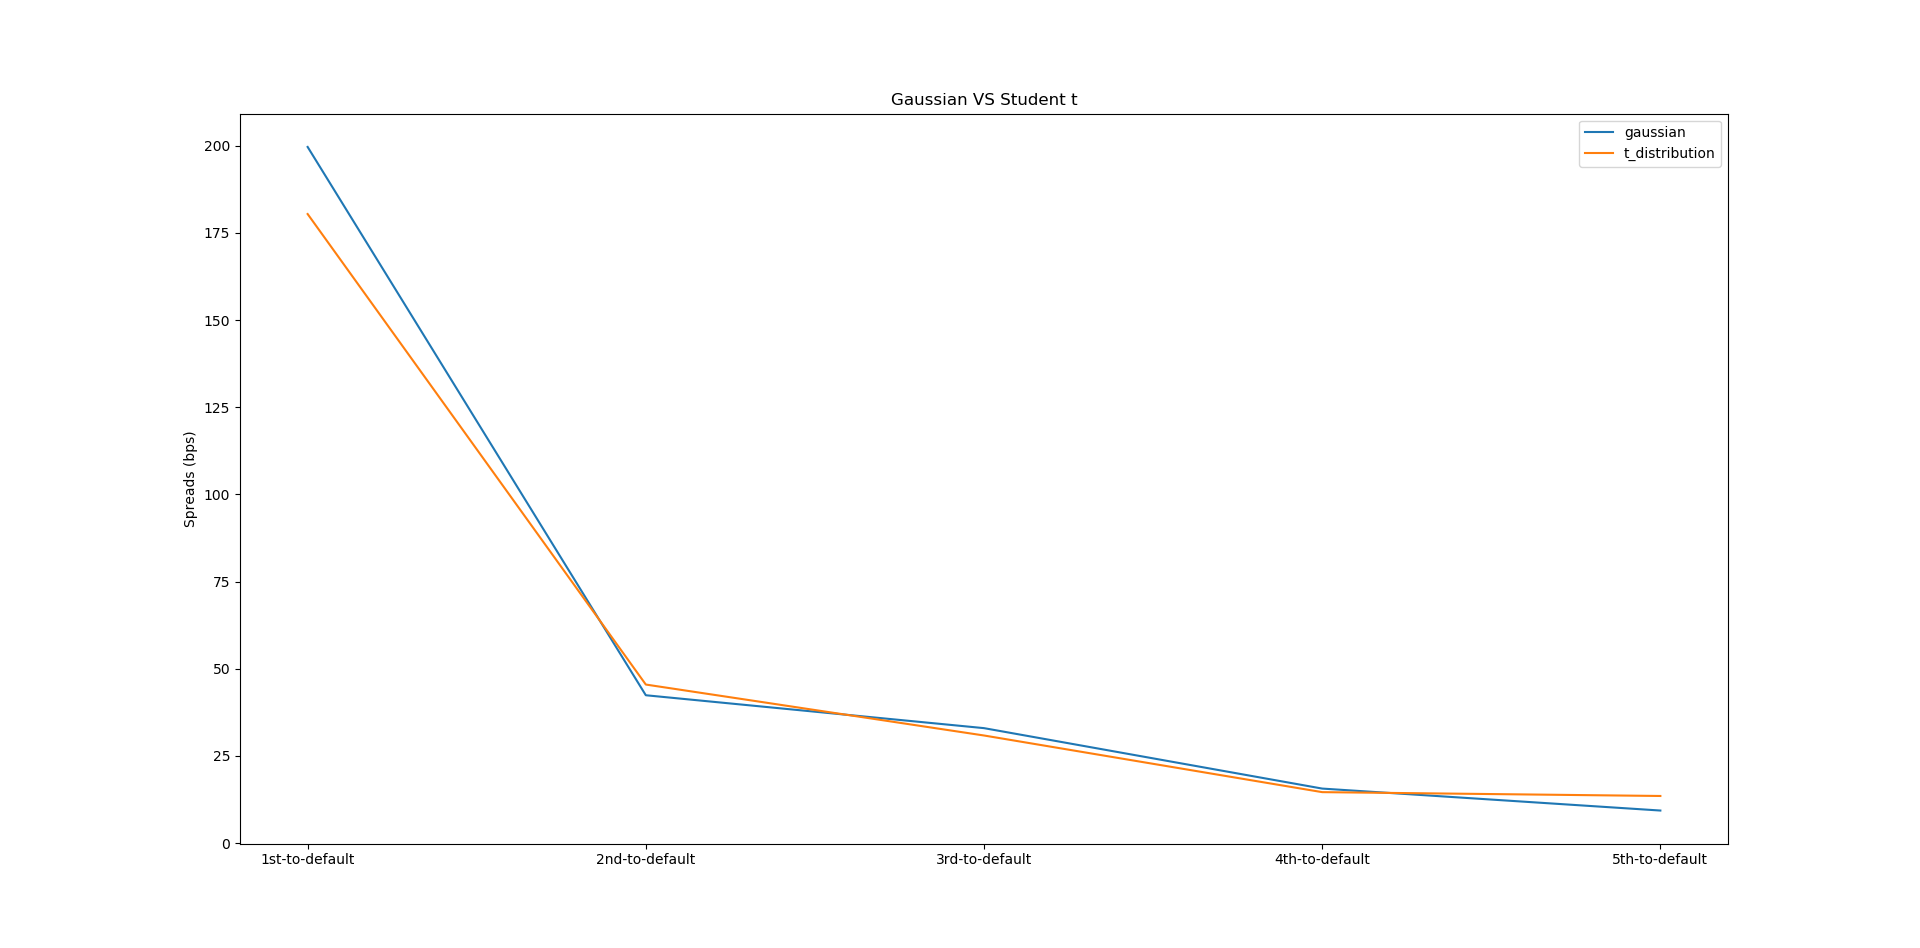
\includegraphics[width=1\textwidth]{tstat_vs_gaussian}
\caption{Comparison of t distribution vs Gaussian}
\label{image-t_vs_gaus}

\end{figure} 

\clearpage

A first take away is that the prices are almost similiar, too far off would raise warnings about the validity of one over the other. Next, spread drops as one considers less riskier contracts, as expected. 

\subsection{Variance Reduced Monte Carlo}

As one would find, and also included in \cite{joshi_kainth} and \cite{milicia}, the basic Monte Carlo algorithm as outlined above takes slower to converge because most of the path generated lead to $\tau_i$ outside the desired interval $0 < \tau_i \leq T$, hence leading to constant values of the running spread in the loop. To combat this behaviour, one can consider a change of measure, by adjusting the probabilities of default such that $\tau_i < T$ is always achieved on each path.  The details of the algorithm are included in the original texts by the various authors, but below is a sketch of the idea. This is assuming algorithm for the gaussian copula, 

\begin{align*}
\tau_i < T  & \Leftrightarrow F_i(\tau_i) < F_i(T) \\
 & \Leftrightarrow N^{-1}( F_i(\tau_i)) < N^{-1}(F_i(T)) \\
 & \Leftrightarrow W < X \\
 & \Leftrightarrow AZ < X \\
 & \Leftrightarrow Z_i < \frac{X_i - \sum\limits_{j < i}A_{ij}Z_j}{A_{ii}} \\
 & \Leftrightarrow N(Z_i) < N\left(\frac{X_i - \sum\limits_{j < i}A_{ij}Z_j}{A_{ii}} \right) \\
 & \Leftrightarrow v_i < p_i .
\end{align*}

This working simply  shows that it is possible from randomly drawn uniform variates $v_i$ to impose some conditions on them so as to ensure that the final obtained $\tau_i \leq T$ and hence a default is observed. However, as noted by \cite{milicia}, this comes at a computational costs nut definitely gives results for less simulated paths. The variance reduction method worlks particularly well in the rare case of payoff by a 5th-to-default basket, where all names have to default within the maturity $T$. 
Below is a plot showing the convergence of a 1st-to-default basket CDS computed using the reduced variance algorithm. 

\begin{figure}[h]

\centering
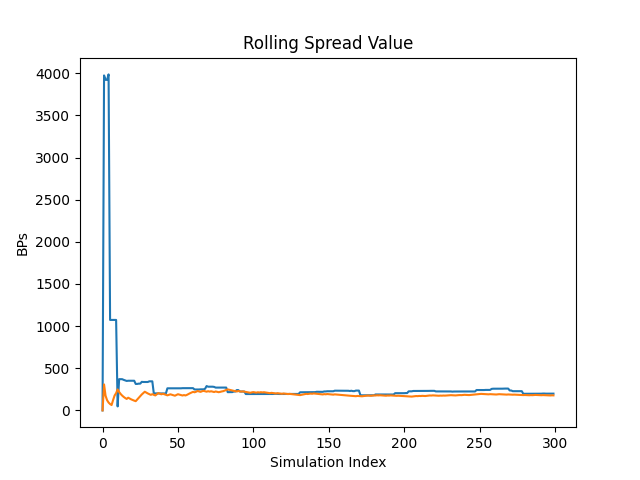
\includegraphics[width=0.8\textwidth]{rolling_spread_mc}
\caption{Adjusted MC vs Plain MC for 1st-to-default CDS}
\label{image-adjusted_vs_plain_mc}

\end{figure}

As can be seen from the graph, both algothim seem to converge at one value after about 275 runs. The graph shows the spread value calculated after each run, taking into account the changing premium/protection legs. The blue graph is for the adjusted algorithm. The copula used was the gaussian copula. The plot shows how quickly the adjusted MC method stabilizes and continues with little variance. The 1st-to-default case is not ideal for demonstrating the usefulness of the adjusted method; one would need to compare the 5th-to-default case. However, that comes at a cost on the number of runs needed to see converge for the plain MC method.  

\clearpage

\subsection{Copula Fitting and Default Correlation Matrix}
The correlation matrix is an important parameter into the pricing of a basket CDS, and it can bring about significant model risk in the pricing. Proper fitting has to be done in order to ensure the output spreads are correct. However, this task is not so straightforward. As mentioned in the various cited texts, the choice of correlation measure is of great importance as other choices can lead to misinterpretation of the core correlation of defaults. The linear correlation is one such example, while it works well for a gaussian copula, it does not do so great when it comes to non-normal distribution like the student's t distribution. In practice, one is faced with the formidable task of estimating the correct correlation matrix for the observed distribution. The first step towards achieving this is a simple test of uniformity of the implied cdf from the historical data. This can be done through libraries such as kernel density approximation. The results shown below depicts the outcome of such a method.

\begin{figure}[h]

\centering
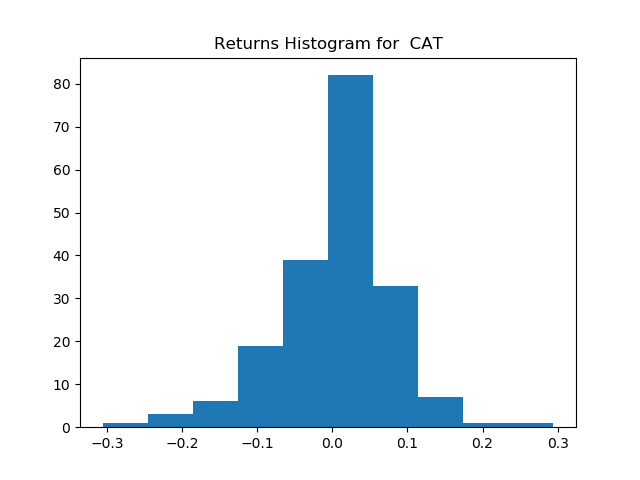
\includegraphics[width=0.5\textwidth]{cat_returns_histogram}
\caption{Returns Histogram for company CAT}
\label{image-cat_hist}

\end{figure} 

\begin{figure}[h]

\centering
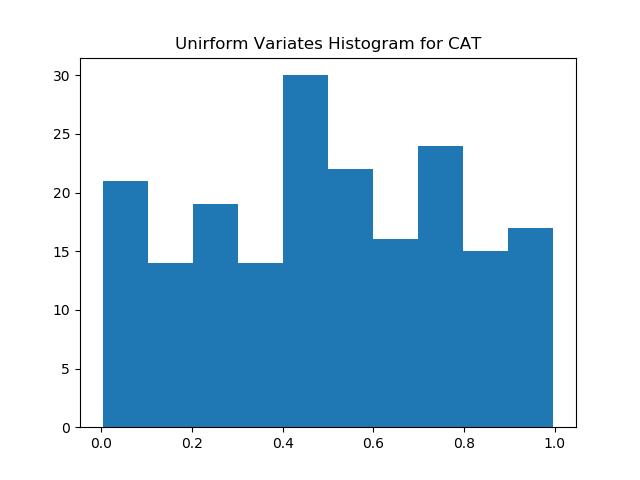
\includegraphics[width=0.5\textwidth]{cat_uniforms_histogram}
\caption{Uniforms Histogram for company CAT}
\label{image-cat_hist1}

\end{figure} 

\begin{figure}[h]

\centering
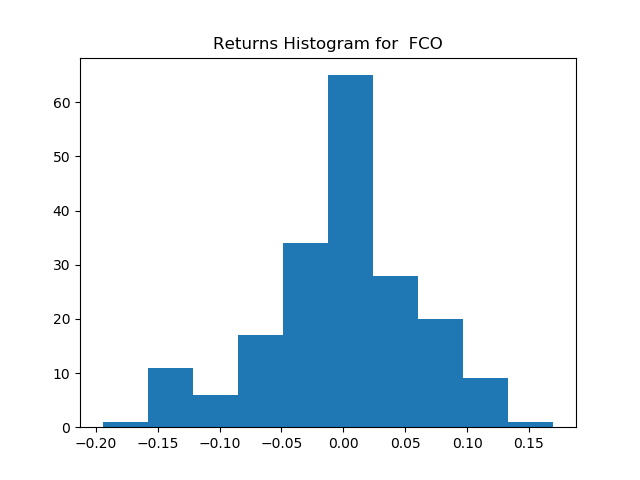
\includegraphics[width=0.5\textwidth]{fco_returns_histogram}
\caption{Returns Histogram for company FCO}
\label{image-fco_hist}

\end{figure} 

\begin{figure}[h]

\centering
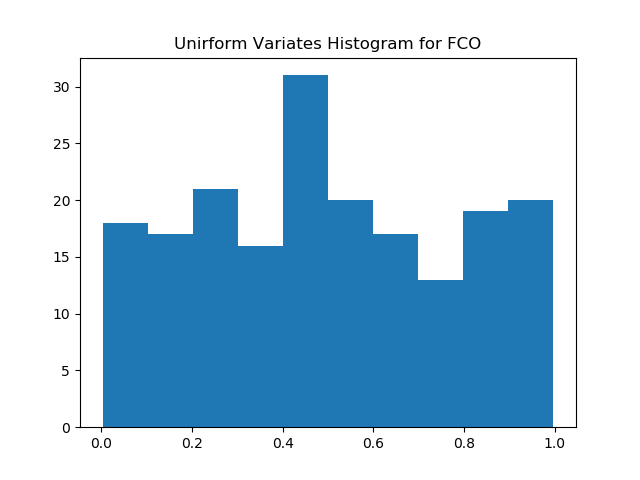
\includegraphics[width=0.5\textwidth]{fco_uniforms_histogram}
\caption{Uniforms Histogram for company FCO}
\label{image-fco_hist1}

\end{figure} 

\begin{figure}[h]

\centering
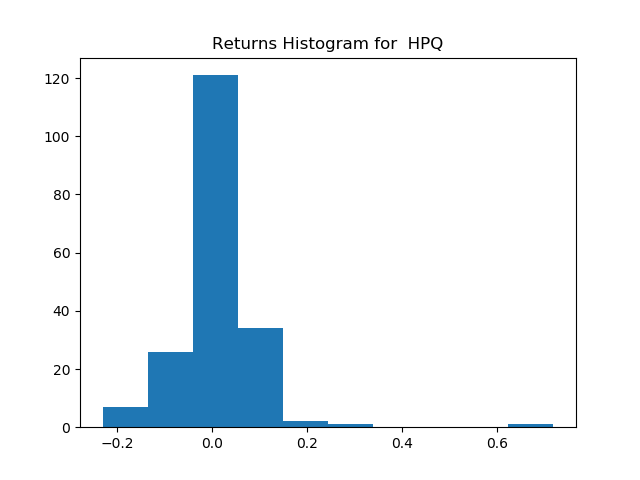
\includegraphics[width=0.5\textwidth]{hpq_returns_histogram}
\caption{Returns Histogram for company HPQ}
\label{image-hpq_hist}

\end{figure} 

\begin{figure}[h]

\centering
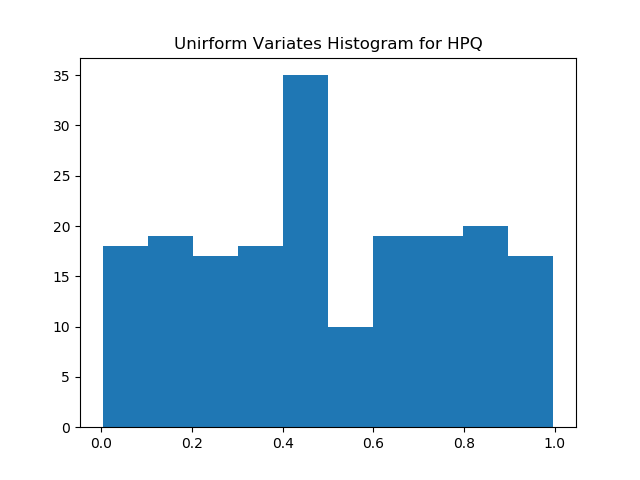
\includegraphics[width=0.5\textwidth]{hpq_uniforms_histogram}
\caption{Uniforms Histogram for company HPQ}
\label{image-hpq_hist1}

\end{figure}

\begin{figure}[h]

\centering
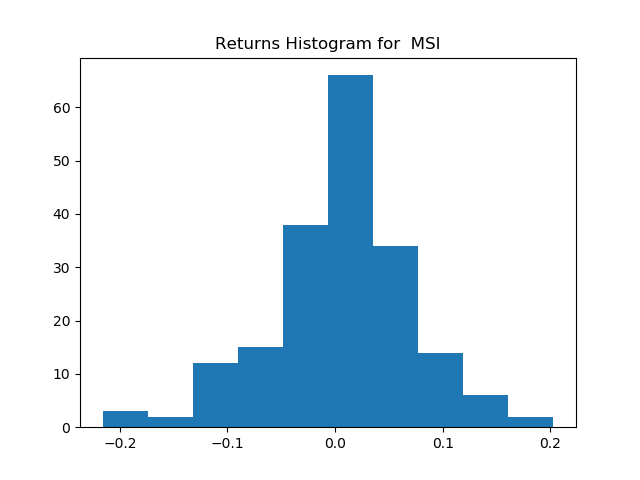
\includegraphics[width=0.5\textwidth]{msi_returns_histogram}
\caption{Returns Histogram for company MSI}
\label{image-msi_hist}

\end{figure} 
 
\begin{figure}[h]

\centering
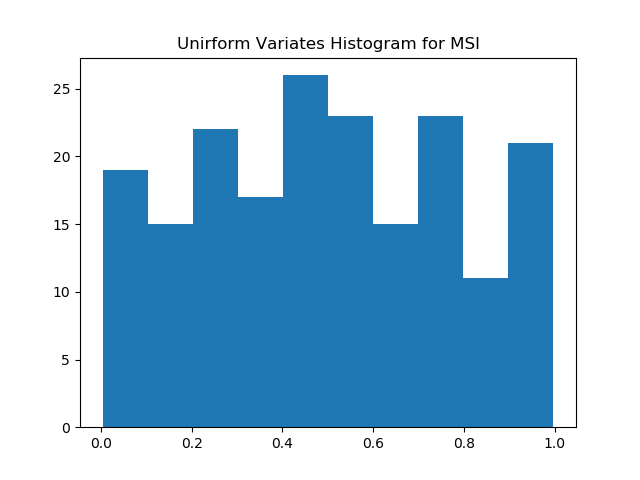
\includegraphics[width=0.5\textwidth]{msi_uniforms_histogram}
\caption{Uniforms Histogram for company MSI}
\label{image-msi_hist1}

\end{figure} 
 
\begin{figure}[h]

\centering
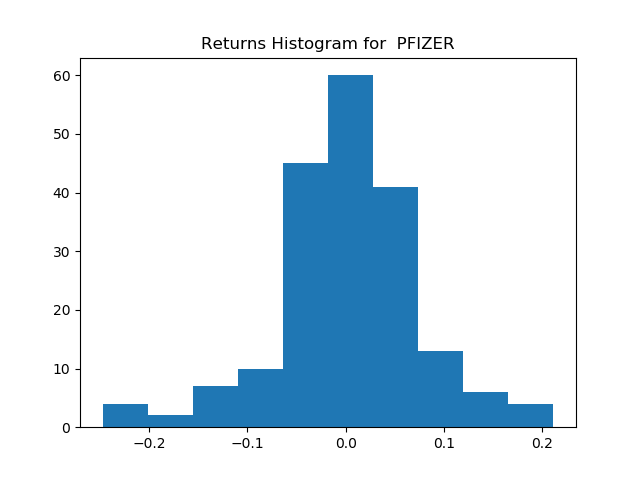
\includegraphics[width=0.5\textwidth]{pfizer_returns_histogram}
\caption{Returns Histogram for company PFIZER}
\label{image-pfizer_hist}

\end{figure} 
 
\begin{figure}[h]

\centering
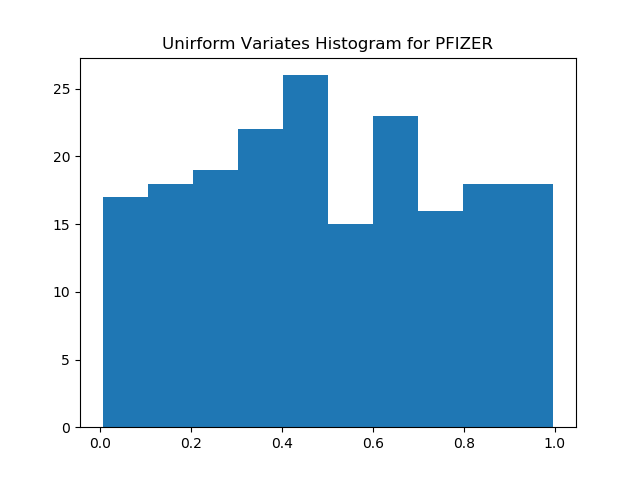
\includegraphics[width=0.5\textwidth]{pfizer_uniforms_histogram}
\caption{Uniforms Histogram for company PFIZER}
\label{image-pfizer_hist1}

\end{figure} 


\clearpage

As can be seen from the plots, the kernel density approximation method did not output completely uniform pseudo-samples, but there was a noticeable effect of the method. The method employed directly gives out the implied cdf, though this may include some approximation done internally by the functions built within the package. One resolution of this would be to pursue the scikit-learn route which only estimates the pdf, then one would perform numerical integration to obtain the cdf. This incomplete uniformity might be the cause of other incorrect model output to be discussed next. Obtaining the psuedo-samples is only the first step towards obtaining an estimate for the correlation. The next step is to use the linear correlation formula on the pseudo-samples, which is effectively giving the Spearman's rho, a rank correlation. The Spearman's rho can be "linearized" using $\rho = 2sin\left( \frac{\pi}{2}\rho_s\right)$. The result can be checked for positive definiteness through its eigenvalues, and if any one of these is negative, a close positive number is obtained in order to transform the matrix to positive definite as required for Cholesky decomposition in the MC algorithm.
\newline
Having found the rank correlation, and estimated the correlation matrix, there is still one more step to go to complete the fitting (in the case of t copula). The degrees of freedom paramaters still needs to be estimated through MLE techniques. The approach taken was to use the equation for the pdf for multivariate t copula and maximize the log-likelihood as a function of $\nu$ when given the correlation matrix $\Sigma$. However, as can be seen from the graph below, such a maximizing $\nu$ was not found. The log-likelihood exhibited unfamiliar behaviour of an ever increasing function.

\begin{figure}[h]

\centering
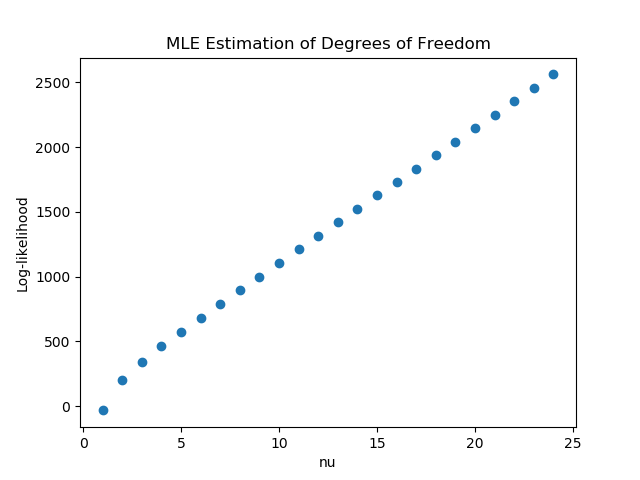
\includegraphics[width=0.5\textwidth]{mle_approximation_df}
\caption{MLE Estimation for $\nu$ Trial}
\label{image-mle}

\end{figure} 
 
The simpler method, as demonstrated in the workshop, was to take the degrees of freedom simply as 9 since none of the pairs demonstrated high correlation coefficients. 

\subsection{Risk and Sensitivity Analysis}
The section covers sensitivity analysis of the spread with respect to certain important parameters in the pricing. The first is the sensitivity to recovery rate (this has been considered constant throughout the project, though possible extensions would be to allow for it to vary stochastically), the second is sensitivity with respect to hazard rates/spreads. This has been tackled in \cite{joshi_kainth} and \cite{peter_jackel} at some detail. The last is the sensitivity to default correlation, $\Sigma$, which is tackled here through stress-testing at high/low values, corresponding to perfect correlation/independent cases. The plot belows demonstrate the behaviour of spreads against low/high correlation values. The pair-wise correlation coefficient is assmued the same for all possible pairs.

\begin{figure}[h]

\centering
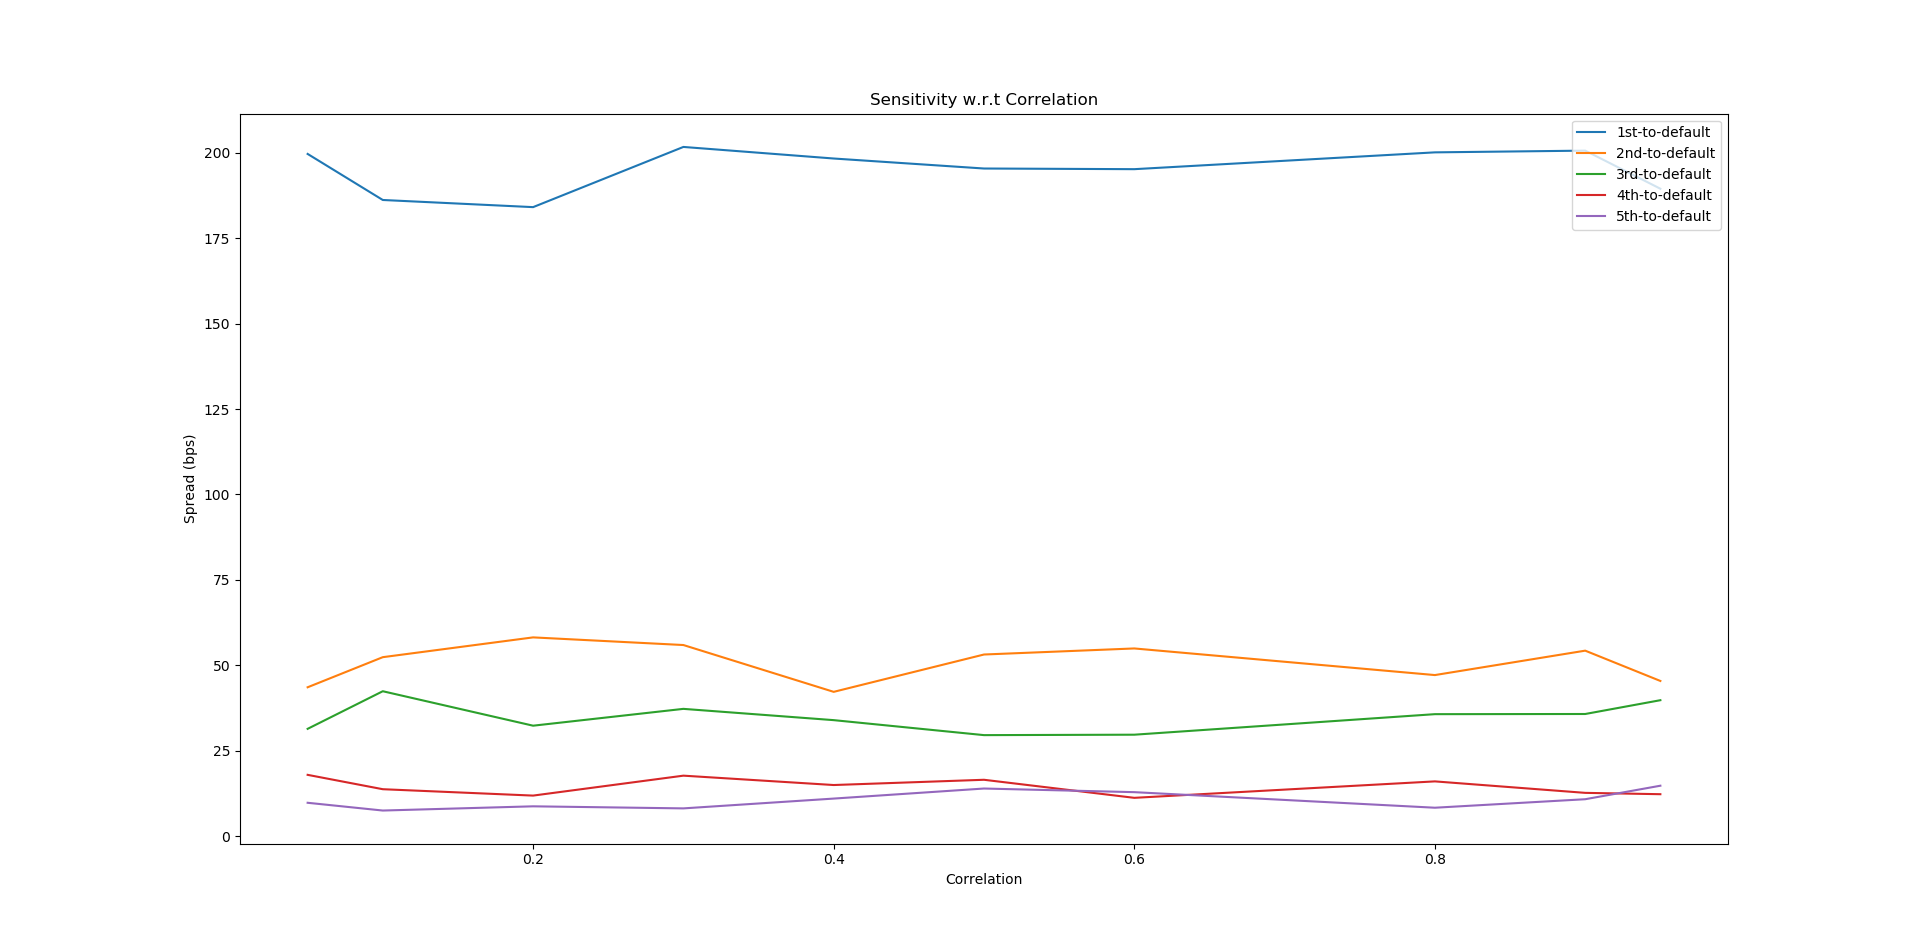
\includegraphics[width=1\textwidth]{sensitivity_wrt_correlation}
\caption{Sensitivity of Spread to Correlation $\rho$}
\label{image-sens_rho}

\end{figure} 

The plot depicts a general observation, the 1st-to-default contract behaving differently than the others. The expected shape is a downward sloping curve as $\rho$ increases from 0.05 to 0.95, however this was not observed, perhaps highlighting an issue with how the correlation matrix was estimated at first.The 5th-to-default contract is correctly below the rest as it is more unlikely that all 5 names default within a given maturity. The intermediate contracts are ordered as expected, 2nd-to-default higher than 3rd-to-default, which in turns is higher than 4th-to-default contract. 
\newline
The other sensitivity to explore is with respect to the recovery rate (i.e LGD). This was computed readily by picking plausible values for the LGD in the range (0, 1). The plot provided gives an indication of the dependency on LGD.

\begin{figure}[h]

\centering
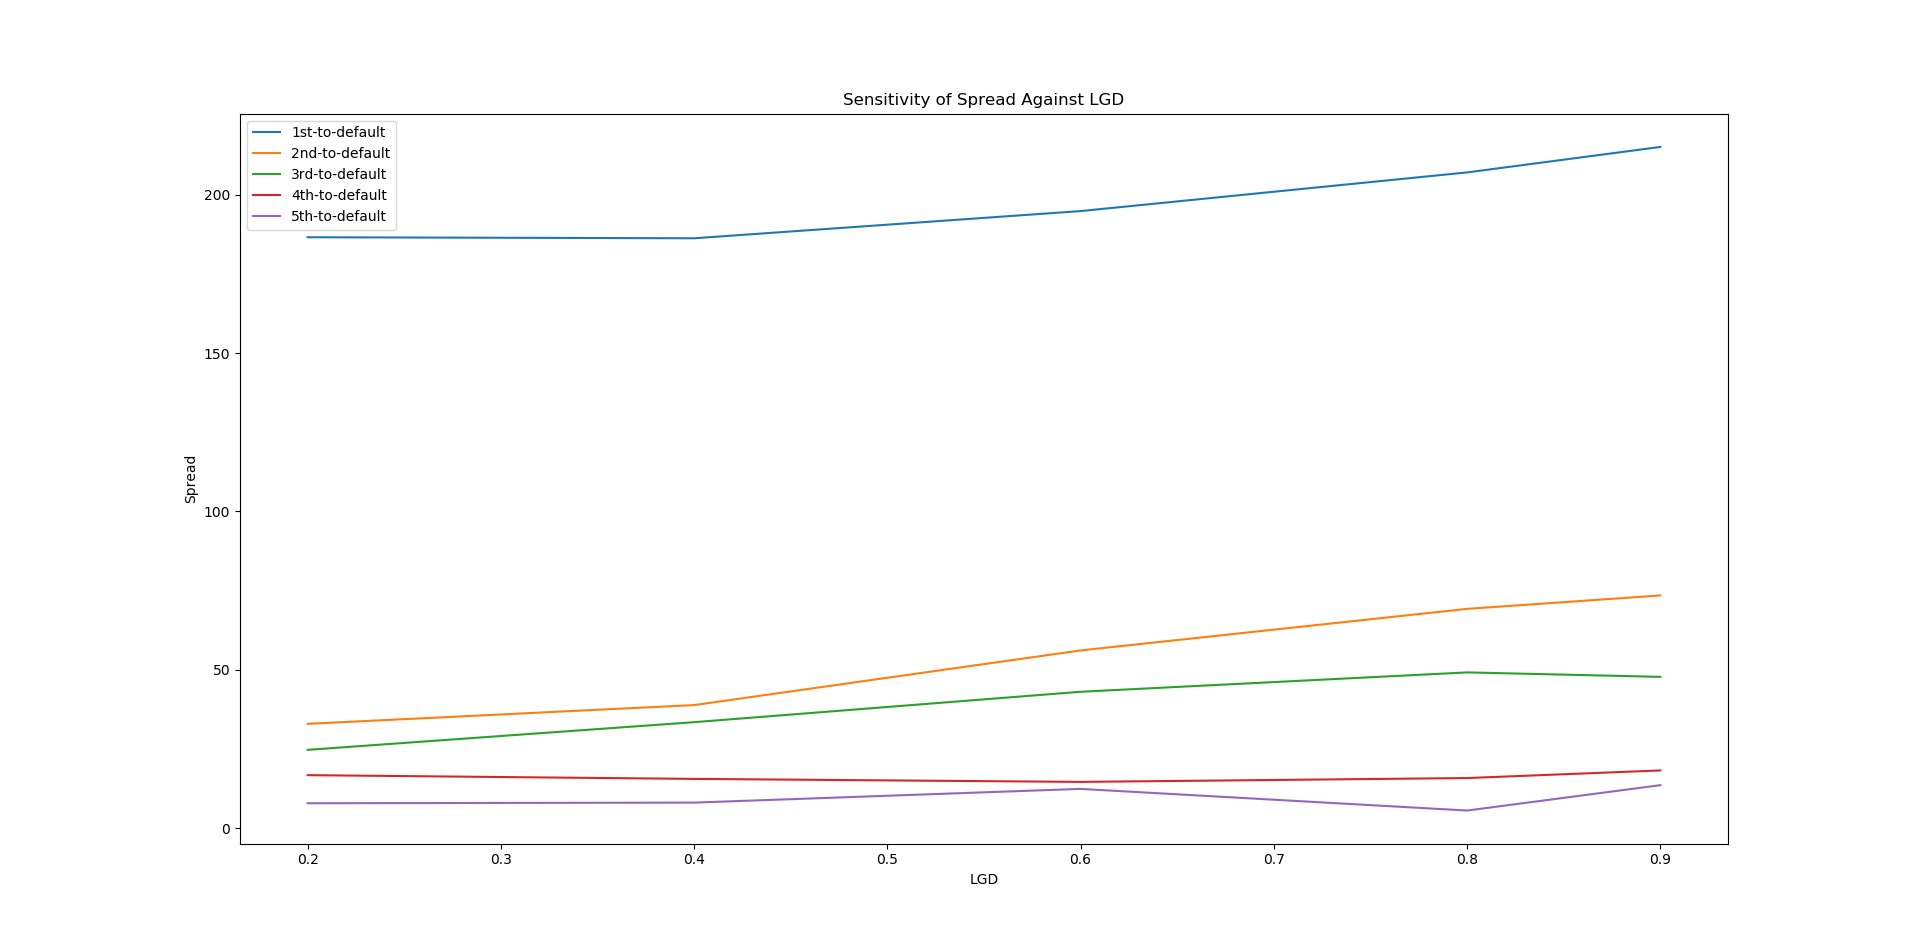
\includegraphics[width=1\textwidth]{sensitivity_wrt_lgd}
\caption{Sensitivity of Spread to LGD}
\label{image-sens_lgd}

\end{figure} 

intuitively, one would expect the spreads to increase as the LGD increases, and this is what is depicted in the figure.Again the order is preserved, 1st-to-default is more riskier (higher spread) than all the others, and 5th-to-default is less riskier than the others. 
\newline
The sensitivity with respect to spread/hazard rates is a challenging one to compute. Monte Carlo techniques are well known to fall short in this regard, however there are specialized techniques that can be employed to compute greeks for the basket CDS product. The techniques are not only limited to basket CDS however. As explained in \cite{joshi_kainth} and \cite{peter_jackel}, there are a few methods devoted to computing greeks of derivatives products, nonetheless this project only focused on one, namely the likelihood ratio method. Suppose $V$ is the value of a contingent claim, the text by \cite{joshi_kainth} showed a way of computing the $\frac{\partial V}{\partial h_i}$ where $h_i$ is a constant hazard rate. The resulting equation was given by 

\begin{equation}
\frac{\partial V}{\partial h_i} = \int B(\tau_1, \tau_2, \dots, \tau_n)\frac{\partial log\phi(\tau_1, \tau_2, \dots, \tau_n)}{\partial h_i}\phi(\tau_1, \tau_2, \dots, \tau_n)d\tau_1 d\tau_2 \dots d\tau_n
\end{equation}

where 

$$ \frac{\partial log\phi(\tau_1, \tau_2, \dots, \tau_n)}{\partial h_i} = \sum_{j}(\mathbf{\Sigma}^{-1} - \mathbf{1})_{ij}\nu_j\frac{\partial \nu_i}{\partial u_i}\frac{\partial u_i}{\partial h_i} + \frac{1}{h_i} - \tau_i$$

 and 
$$\frac{\partial \nu_i}{\partial u_i} = \sqrt{2\pi}e^{\frac{1}{2}N^{-1}(u_i)^2}$$

The procedure, then, to compute the sensitivity with respect to hazard rate is simple, as already noted from \cite{joshi_kainth}. The algorithm works hand in hand with the adjusted (importance sampling) technique, and it is the approach used in this project in order to obtain the sensitivities. The table below shows the output from such a computation. 

\begin{table}[h!]
\begin{center}
\begin{tabular}{ |c|c|c|c|c|c| }

\hline
 &$ A_1 $ & $ A_2 $ & $ A_3 $ & $ A_4 $ & $ A_5 $\\
\hline
1st-to-default & 42.7 & 300.8 & 160.2 & 188.9 & -2667.9 \\ 
\hline
2nd-to-default & 101.6 & 341.3 & 274.4 & 285.9 & -2746.9 \\
\hline
3rd-to-default  & 16.48 & 29.6 & 37.6 & 34.6 & -194.7 \\
\hline
4th-to-default  & 7.22 & 6.5 & 14.6 & 12.34 & -24.8 \\
\hline
5th-to-default  & 0.105 & 0.034 7 & 0.197 & 0.154 & 0.217 \\
\hline

\end{tabular}
\caption{Sensitivities of Spread's Against Hazard Rates of Names in the Basket}
\end{center}
\end{table}

The table is showing sensitivities of each CDS type against average hazard rate for each name. First-to-default swaps are the most affected by a change in hazard rates of one name, intuitively this is to be expected as one credit rating changes, that one name's $\tau_i$ will change, thereby altering the nth-to-default time. First-to-default is affected positively for the most names, except one. As we move away from 1st-to-default type, the sensitivities drop, with the 5th-to-default offering very small sensitivies to any one of the name. Intuitively, a change in credit by one of the names offers little change to the overall default probability of all names, here it is assumed changes are all happening one at a time.

\section{Conclusion}
Numerous aspects of Monte Carlo pricing were studied in this project. The first was the role of different distributions to the spread output. The evidence suggest that t distribution spreads are less than that from gaussian, on average. One property of the t distribution is that if $u \approx 0.1$ then $v \approx 0.1$ almost surely. This has great effect on simulated default times and could be given also as an explanation as to the difference in prices between t distribution and gaussian. The other aspects related to the variance reduction in spreads output. For most of the simulated paths, only a fraction will lead to a non-zero payoff. This is affected by the maturity of the contract as well. A short maturity means a smaller fraction of the simulated paths will be significant in the calculation of the spread. These lead to large variances in the rolling premium/protection legs. One approach to reduce this variance is through likelihood ratio (also referred in the literature as importance sampling). This aims to ensure for every generated pseudo uniform $u_i$, the default time $\tau_i$ falls within the maturity $T$. With some alterations to the original code, it is possible to accomodate this scheme. This turned out to work quite well for the rare case scenario of the 5th-to-default contract. In fact, as already mentioned in the literature, \cite{peter_jackel}, this method is also used for deep out of the money options. Importance sampling also becomes extremely useful in the computation of the 'greek', senstivity to hazard rates. The drawback with this technique is the additional computation time taken as numerous conditions are put in place on each random draw of $u_i$. A lot more calculation goes on internally before the spread is output. Proper functioning of the likelihood ratio technique requires proper coding and attention to detail. One aspect that was not attempted is the use of pseudo random numbers instead of low discrepancy numbers. This is one topic of interest to be tackled at a later stage. The biggest challenge in the project was the fitting of the copula to data. Default correlation plays an important role in credit portfolio modelling and as a result great effort should be put in order to estimate it satisfactorily. The section on this topic highlighted some pitfalls. Though the uniformity check was not one hundred percent successful, it was not entirely futile. There was a degree of conversion from normal variates to pseudo-uniform samples. The correlation matrix obtained was through spearman's rho, and this was linearized according to literature standard. Computation of the degrees of freedom parameter proved intractable. The explicit MLE approach did not yield expected behaviour consequently leading to the adoption of a simpler estimate to the degrees of freedom. The last section focused on sensitivity calculations. The sensitivity plot for correlation density gives a general expected behaviour. First-to-default swap having a higher spread than the others, and 5th-to-default having the lowest spread than all. However, the expected curvature is not visible from the plot. The simplifying assumption made was to assume all name pairs have the same correlation coefficient, and this was varied from close to zero (nearly independent) to close to one (perfectly correlated).The calculation was done using the plain Monte Carlo algorithm which as already mentioned, has a high variance. The plot of sensitivity against LGD gave expected results, all contracts increasing in spread as the LGD increases. The last sensitivity considered was the change of spread against hazard rate. This gave a general picture that the more riskier contract (1st-to-default) has a high sensitivity against the hazard rate of any one of the names, whereas the less riskier contract (5th-to-default) has relatively low sensitivity against any one given name. 


\medskip

\begin{thebibliography}{20}
\bibitem{paul_wilmott}
Paul Wilmott.
\textit{Paul Wilmott on Quantitative Finance},
John Wiley \& Sons, Ltd, Chapter 41.

\bibitem{peter_jackel}
Peter Jackel.
\textit{Monte Carlo Methods in Finance},
John Wiley \& Sons, Ltd, Chapters 2 \& 9.

\bibitem{credit}
Christian Bluhm, Ludger Overbeck, \& Christoph Wagner.
\textit{An Introduction to Credit Risk Modeling}
Chapman \& Hall, Chapters 6 \& 7.

\bibitem{Antulio}
Antulio N. Bomfim.
\textit{Understanding Credit Derivatives and Related Instruments}
Elsevier Academic Press, Chapters 9 \& 15 \& 20. 

\bibitem{joshi_kainth}
Mark S. Joshi and Dherminder Kainth.
\textit{Rapid and Accurate Development of Prices and Greeks for nth to Default Swaps in the Li Model}, \(2004\).

\bibitem{milicia}
Giuseppe Milicia.
\textit{A Monte Carlo Pricing Engine for nth to Default Credit Swaps in the Li Model},

\bibitem{li_2000}
David X. Li.
\textit{On Default Correlation: A Copula Function Approach}, \(2000\), RiskMetric. 

\bibitem{sergei}
Sergie Winitski.
\textit{A Handy Approximation for the Error/Inverse Function}
\texttt{https://www.academia.edu/9730974/A\_handy\_approximation\_for\_the\_error\_function\_and\_its\_inverse}

\bibitem{mimirgames}
Inverse Error Function link:
\newline
\texttt{http://www.mimirgames.com/articles/programming/approximations-of-the-inverse-error-function/}

\bibitem{dlmf}
Incoplete Beta Function links
\newline
\texttt{https://dlmf.nist.gov/8.17}
\newline
\texttt{https://dlmf.nist.gov/15.2\#i}


\end{thebibliography}

\end{document}